%% ****** Start of file template.aps ******%
%%
%%
%%   This file is part of the APS files in the REVTeX 4 distribution.
%%   Version 4.0 of REVTeX, August 2001
%%
%%
%%   Copyright (c) 2001 The American Physical Society.
%%
%%   See the REVTeX 4 README file for restrictions and more information.
%%
%
% This is a template for producing manuscripts for use with REVTEX 4.0
% Copy this file to another name and then work on that file.
% That way, you always have this original template file to use.
%
% Group addresses by affiliation; use superscriptaddress for long
% author lists, or if there are many overlapping affiliations.
% For Phys. Rev. appearance, change preprint to twocolumn.
% Choose pra, prb, prc, prd, pre, prl, prstab, or rmp for journal
%  Add 'draft' option to mark overfull boxes with black boxes
%  Add 'showpacs' option to make PACS codes appear
%  Add 'showkeys' option to make keywords appear
%\documentclass[aps,prl,preprint,groupedaddress]{revtex4}
\documentclass[preprint,authoryear,12pt]{elsarticle}
%\documentclass[aps,prl,twocolumn,groupedaddress]{revtex4}
\usepackage{amssymb}
\usepackage{amsmath}
\usepackage{multirow}
\usepackage{dsfont}
\usepackage{graphicx}
\usepackage{rotating}
\usepackage{sidecap}
\usepackage{tabularx}
% You should use BibTeX and apsrev.bst for references
% Choosing a journal automatically selects the correct APS
% BibTeX style file (bst file), so only uncomment the line
% below if necessary.
%\bibliographystyle{apsrev}

\begin{document}

% Use the \preprint command to place your local institutional report
% number in the upper righthand corner of the title page in preprint mode.
% Multiple \preprint commands are allowed.
% Use the 'preprintnumbers' class option to override journal defaults
% to display numbers if necessary
%\preprint{}

%Title of paper
\title{Sloppy-Stiff Supplementary addition: Nutrient Model}

% repeat the \author .. \affiliation  etc. as needed
% \email, \thanks, \homepage, \altaffiliation all apply to the current
% author. Explanatory text should go in the []'s, actual e-mail
% address or url should go in the {}'s for \email and \homepage.
% Please use the appropriate macro foreach each type of information

% \affiliation command applies to all authors since the last
% \affiliation command. The \affiliation command should follow the
% other information
% \affiliation can be followed by \email, \homepage, \thanks as well.
\author[physics]{Bradford P. Taylor}
%\email[]{Your e-mail address}
%\homepage[]{Your web page}
%\thanks{}
%\altaffiliation{}
\address[physics]{School of Physics, Georgia Institute of Technology, Atlanta, GA, USA}

%Collaboration name if desired (requires use of superscriptaddress
%option in \documentclass). \noaffiliation is required (may also be
%used with the \author command).
%\collaboration can be followed by \email, \homepage, \thanks as well.
%\collaboration{}
%\noaffiliation

\date{\today}

% insert suggested PACS numbers in braces on next line \pacs{}
% insert suggested keywords - APS authors don't need to do this
%\keywords{}

%\maketitle must follow title, authors, abstract, \pacs, and \keywords
\maketitle

% body of paper here - Use proper section commands
% References should be done using the \cite, \ref, and \label commands
\section{Sloppy-Stiff}
% Put \label in argument of \section for cross-referencing
%\section{\label{}}
In general, perturbing parameter values in a model can have different effects on the output. Parameters upon which perturbations cause large (small) changes to output are referred to as stiff (sloppy). If one considers small perturbations to a predetermined reference set of parameters the entire information of sloppy-stiffness is contained within the parametric Hessian matrix, where the $ij$th element is commonly defined in a unitless fashion (cite gutenkunst) :

\begin{eqnarray}
H_{ij} = \sum_{n} \frac{\partial{\log{y_n}}}{\partial{\log{\theta_i }}}\bigg|_{\vec \theta^*} \frac{\partial{\log{y_n}}}{\partial{\log{\theta_j}}}\bigg|_{\vec \theta^*} = \sum_{n} \frac{\theta^*_i \theta^*_j}{(y^*_n)^2} \frac{\partial y_n}{\partial{\theta_i}}\bigg|_{\vec \theta^*} \frac{\partial y_n}{\partial{\theta_i}}\bigg|_{\vec \theta^*}.
\end{eqnarray}

Above, there are a total $n$ total variables in the model and the reference parameters are represented by a vector $\vec \theta$. The bar notation emphasizes that the partial derivatives are evaluated at the reference parameter set. The argument of the sum is made unitless by a prefactor involving the reference parameter set and the respective equilibrium values of the variables, $\vec y^*$. Each element of the hessian is interpreted as the sum of the relative changes of each variable due to relative changes of the respective parameters.

Eigenvalues of the Hessian quantify the total amount of change to all variables given a perturbation to a combination of parameters defined by the respective eigenvector. The eigenvalue spectrum shows that perturbations to some combinations of parameters cause a majority of the effect on variables. The following figure shows the eigenvalue spectrum for the maximum 10 eigenvalues where the largest value is normalized to 1. For our analysis, we considered perturbations to all parameters except $p_g$, $p_{on}$, and $p_{in}$ due to the algebraic constraint imposed by conservation of mass.

\begin{figure}[h!]
    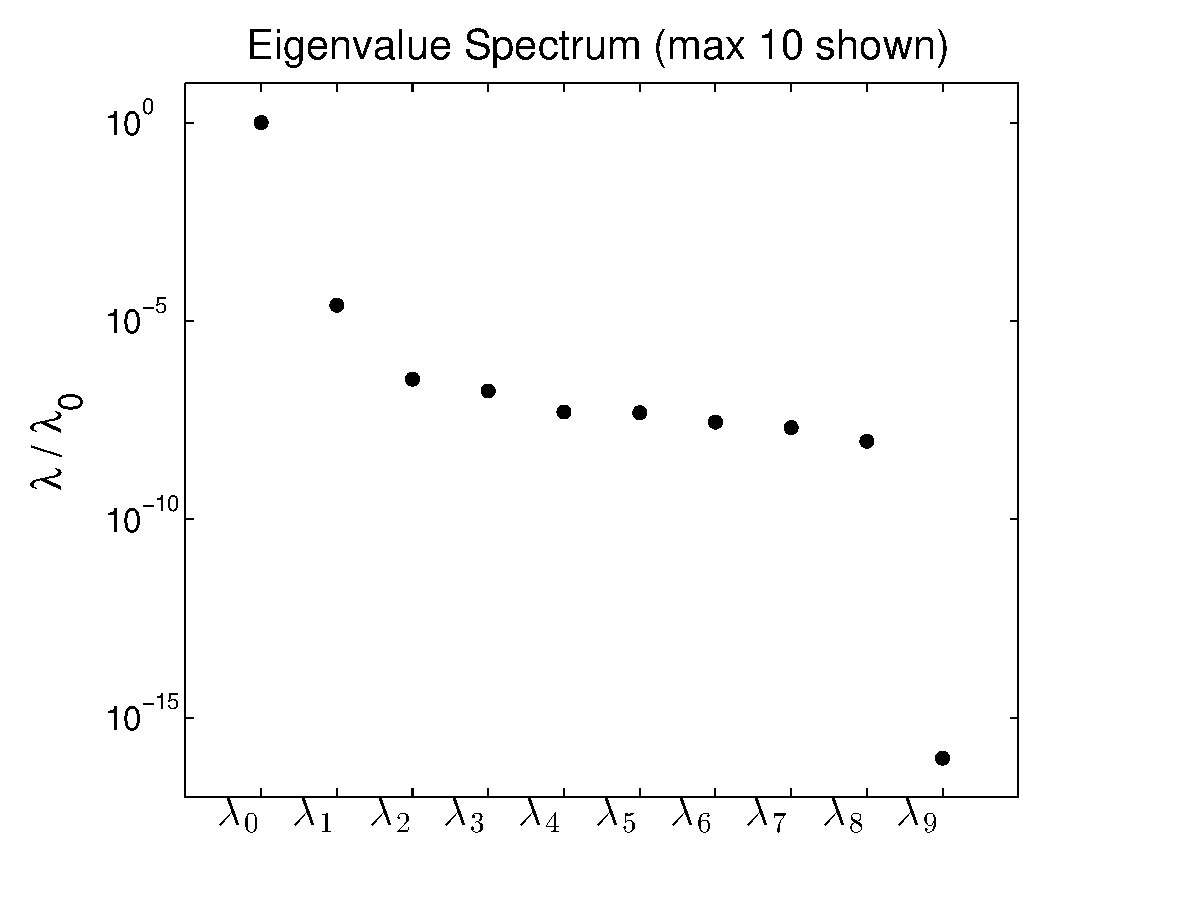
\includegraphics[width=0.75\textwidth]{figures/eigenvalue.eps}%
      \caption{Eigenvalue Spectrum of parametric Hessian matrix. Values are normalized relative to the principle eigenvalue. Only the first 10 eigenvalues of the spectrum are shown. Analysis done by considering perturbations to all parameters except $p_g$, $p_{on}$, and $p_{in}$.}\label{fig:eigenval} 
\end{figure}


Each eigenvalue corresponds to some combination of parameters. In our case, the eigenvalue spectrum is dominated by the principle eigenvalue. To get a sense of which parameters are stiff and sloppy we look at the orientation of principle eigenvector in parameter space. The following figure shows the values of the eigenvector in raw parameter space in order of decreasing stiffness.

\begin{figure}[h!]
    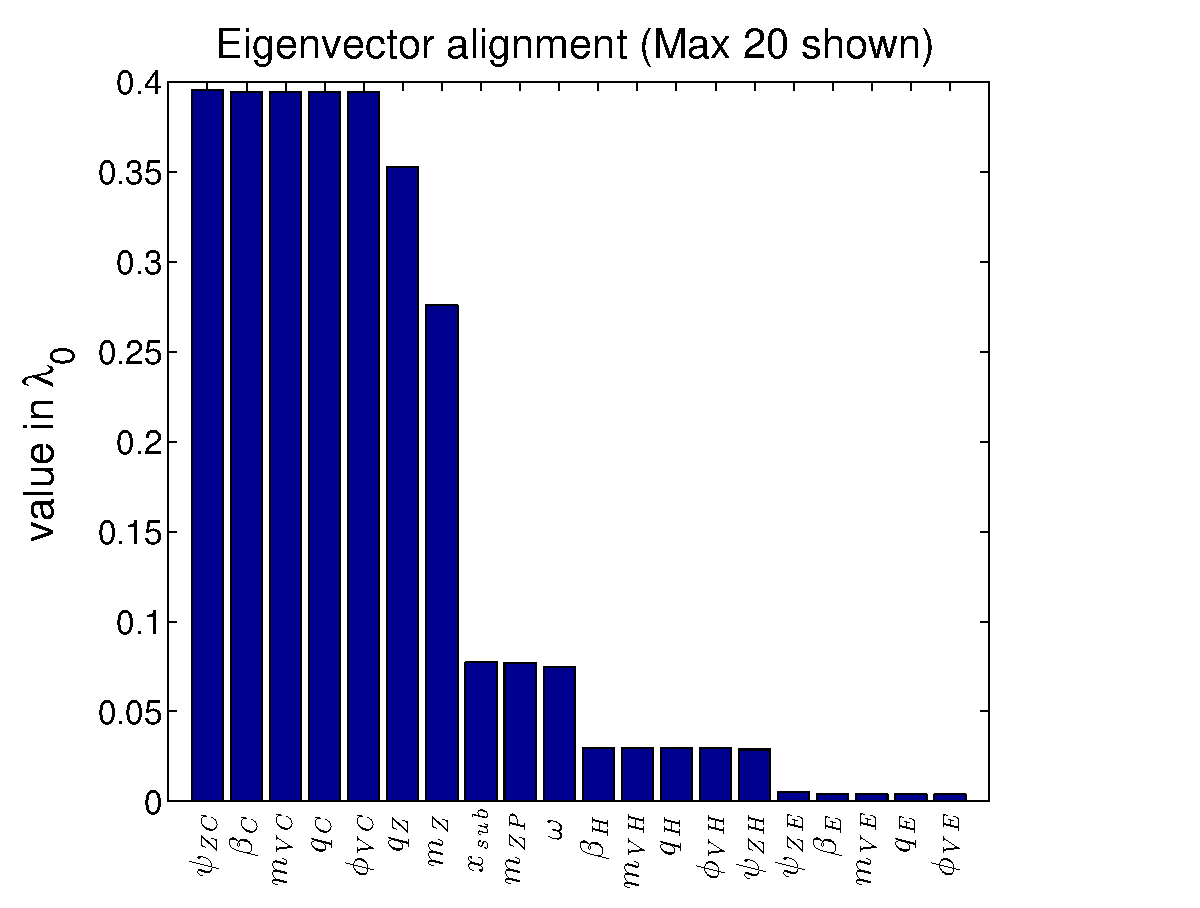
\includegraphics[width=0.75\textwidth]{figures/eigenvector.eps}%
      \caption{Entries of eigenvector. The higher values correspond to stiffer parameters. Only the 20 stiffest parameters are shown.  Analysis done by considering perturbations to all parameters except $p_g$, $p_{on}$, and $p_{in}$.}\label{fig:eigenvec} 
\end{figure}


% Create the reference section using BibTeX:
\bibliography{setup}

\end{document}
%
% ****** End of file template.aps ******


